

\section{Methodology}
\label{sec:method}
In this section, we present the two core concepts of the RiskDreamer framework: batch planning in the latent space and action expansion for balancing entropy and risk, as illustrated in fig. \ref{fig:algo}. Additionally, we introduce the trustworthy traffic scenario generation framework used for training and evaluating autonomous driving agents, as shown in Fig. \ref{fig:calibration}.

\subsection{Framework Overview}

The proposed RiskDreamer framework comprises three interconnected neural networks: a world model for predicting the outcomes of potential actions, a critic network for evaluating the future value of these outcomes, and a policy network for selecting actions that lead to the most valuable results. As the agent interacts with the environment, these components are trained concurrently based on replayed experiences. A central element of our approach is a batch online planner that integrates these three networks. At each decision-making step, this planner initiates a batch rollout using the world model's dynamics model. This process simultaneously explores multiple potential future trajectories within the latent space in a single rollout, offering enhanced planning efficiency. The policy network features an expanded action space, additionally outputting two balancing weights. These weights dynamically adjust the influence of expected rewards, entropy, and risk aversion at each step, derived from the world model's predictions. This transforms what are typically manually tuned hyperparameters into learnable, context-dependent strategies, enabling the agent to adapt its risk tolerance and exploration strategy according to the prevailing traffic conditions. This contrasts with other methods that rely on fixed hyperparameters, allowing for greater adaptability and potentially improved performance in complex and uncertain environments. We will now delve into the specifics of these components and their interactions.

\subsection{Preliminaries from DreamerV3}

RiskDreamer builds upon the foundation of the DreamerV3 world model. As depicted in Fig. \ref{fig:algo} (a), at each time step $t$, the world model receives an observation $\mathbf{o}_t$ and an action $\mathbf{a}_t$ as input. First, an observation encoder $\phi_{\text{enc}}$ maps the observation $\mathbf{o}_t$ to a latent representation $\mathbf{s}_t$:
\begin{equation}
\mathbf{s}_t = \phi_{\text{enc}}(\mathbf{o}_t),
\end{equation}
Given the current latent state $\mathbf{s}_t$ and action $\mathbf{a}_t$, the dynamics model $\phi_{\text{dyn}}$ predicts the next latent state $\widetilde{\mathbf{s}}_{t+1}$. The dynamics model is typically composed of a deterministic component and a stochastic component. Let $\boldsymbol{h}_t$ denote the deterministic state at time $t$. The dynamics model can be described as follows:
\begin{equation}
    \begin{split}
    \boldsymbol{h}_{t+1} &= f_{\phi}(\boldsymbol{h}_t, \mathbf{s}_t, \mathbf{a}_t), \\
    \widetilde{\mathbf{s}}_{t+1} &\sim p_{\theta}(\cdot | \boldsymbol{h}_{t+1}),
    \end{split}
\end{equation}
where $f_{\phi}$ is a deterministic function learned from $\phi_{\text{dyn}}$, and $p_{\theta}$ represents a probabilistic distribution parameterized by $\theta$. The posterior distribution of the latent state $q_{\phi}(\mathbf{s}_t | \boldsymbol{h}_t, \mathbf{o}_t)$ is inferred by combining the prior $p_{\theta}(\cdot | \boldsymbol{h}_{t})$ from the dynamics model with the current observation $\mathbf{o}_{t}$.

The world model comprises several prediction heads that decode the latent state into different modalities. In addition to the standard decoder for reconstructing the observation, and reward and continue heads from the original DreamerV3, RiskDreamer incorporates a risk prediction head. The outputs of these heads can be expressed as conditional probabilities:
\begin{equation}
    \begin{split}
    \text{Decoder}: \widetilde{\mathbf{o}}_t &\sim {\phi_{\text{dec}}}(\widetilde{\mathbf{o}}_t \mid \mathbf{s}_t), \\
    \text{RewardHead}: \widetilde{\mathbf{r}}_t &\sim {\phi_{\text{reward}}}(\widetilde{\mathbf{r}}_t \mid \mathbf{s}_t), \\
    \text{RiskHead}: \widetilde{\mathbf{\rho}}_t &\sim {\phi_{\text{risk}}}(\widetilde{\mathbf{\rho}}_t \mid \mathbf{s}_t), \\
    \text{ContinueHead}: \widetilde{\mathbf{c}}_t &\sim {\phi_{\text{cont}}}(\widetilde{\mathbf{c}}_t \mid \mathbf{s}_t),
    \end{split}
\end{equation}

where $r_t$ is the reward at time $t$, $\widetilde{\rho_t}$ is the predicted risk, and $c_t$ indicates whether the episode continues at the next step. 
The training of the world model involves minimizing a loss function that includes the reconstruction loss for each head and the KL divergence between the prior and posterior distributions of the latent states.
\begin{algorithm}[H]
    \caption{Batch Planning in Latent Space}
    \label{alg:batch_planning}
    \begin{algorithmic}[1]
    \State \textbf{Input:} Posterior distribution $\mathbf{s}_t$, embedded observation $\mathbf{e}_t$, training flag $\tau$
    \State \textbf{Parameters:} Planning horizon $H$, Batch number $N$
    \State Initialize cumulative value $\mathbb{V}$, entropy $\mathbb{E}$, and risk $\mathbb{R} \gets \mathbf{0}$
    \State Expand $\mathbf{s}_t$ to $N$ simulations: $\mathbf{s}_t \gets \text{expand}(\mathbf{s}_t, N)$
    \For{$t = 1$ to $H$}
        \If{$\tau$ and $t = 1$}  \Comment{Exploration policy}
            \State Sample actions: $\mathbf{a}_t \sim \pi_{\theta_e}(\cdot|\mathbf{s}_t)$ 
            \State Compute log probabilities: $\mathbf{L}_t \gets \log \pi_{\theta_e}(\mathbf{a}_t|\mathbf{s}_t)$
        \Else \Comment{Evaluation policy}
            \State Deterministic action: $\mathbf{a}_t \sim \pi_{\theta_t}(\cdot|\mathbf{s}_t)$ 
            \State Select actions: $\mathbf{a}_t \gets \text{mean}(\pi_{\theta_t}(\cdot|\mathbf{s}_t))$  \Comment{Use the mean of the distribution}
            \State Compute log probabilities: $\mathbf{L}_t \gets \log \pi_{\theta_t}(\mathbf{a}_t|\mathbf{s}_t)$
        \EndIf
        \State Predict next state: $\widetilde{\mathbf{s}}_{t+1} \sim \phi_{dyn}(\mathbf{s}_t, \mathbf{a}_t)$
        \State Predict risk: $\widetilde{\rho}_t \sim \phi_{risk}(\mathbf{s}_t)$
        \State Predict reward: $\widetilde{\mathbf{r}}_t \sim \phi_{rew}(\mathbf{s}_t)$
        \State Estimate policy entropy: $\widetilde{\eta_t} \gets \text{Entropy}(\pi_{\theta_e}(\cdot|\mathbf{s}_t))$
        
        \State Retrieve risk weight \(\omega_{\rho, t}\) and entropy weight \(\omega_{\mathcal{H}, t}\) from the expanded action space.
        \State \(\omega_{\mathcal{H}, t} \gets \text{action}[-1]\)  \Comment{Entropy weight}
        \State \(\omega_{\rho, t} \gets \text{action}[-2]\)  \Comment{Risk weight}
        \State Update cumulative metrics:
        \State $\mathbb{V} \gets \mathbb{V} + \widetilde{\mathbf{r}}_t$, $\mathbb{E} \gets \mathbb{E}$ + $\omega_{\mathcal{H}, t}$ $\cdot$  $\widetilde{\eta_t}$, $\mathbb{R} \gets \mathbb{R} + \omega_{\rho, t} \cdot \widetilde{\rho_t}$
        \State Store actions: $\mathbf{A}_t \gets \mathbf{a}_t$
        \State Update state: $\mathbf{s}_t \gets \mathbf{s}_{t+1}$
    \EndFor
    \State Compute objective: $\mathbf{F} \gets \mathbb{V} + \mathbb{E} + \mathbb{R}$
    \State Select best simulation: $i^* \gets \arg\max(\mathbf{F})$
    \State \textbf{Output:} Best action $\mathbf{a}_{i^*}$, log probability $\mathbf{L}_{i^*}$
    \end{algorithmic}
\end{algorithm}
% The training of the world model involves minimizing a loss function that includes the reconstruction loss for each head and the KL divergence between the prior and posterior distributions of the latent states. The loss function can be expressed as:

% \begin{equation}
%     \begin{split}
%     \mathcal{L}_{WM} = \mathbb{E}_{p_{data}} \Big[
%     & -\log p_{\phi_{\text{dec}}}(\mathbf{o}_t | \mathbf{s}_t)
%     - \log p_{\phi_{\text{reward}}}(r_t | \mathbf{s}_t) \\
%     & - \log p_{\phi_{\text{risk}}}(\rho_t | \mathbf{s}_t)
%     - \log p_{\phi_{\text{cont}}}(c_t | \mathbf{s}_t) \\
%     & + D_{KL}(\underbrace{q_{\phi}(\mathbf{s}_t | \mathbf{s}_{t-1}, \mathbf{a}_{t-1}, \mathbf{o}_t)}_{\text{Posterior}} \\
%     & || \ \underbrace{p_{\theta}(\mathbf{s}_t | \mathbf{s}_{t-1}, \mathbf{a}_{t-1})}_{\text{Prior}})
%     \Big],
%     \end{split}
% \end{equation}
% The KL divergence term encourages the prior distribution of the latent state $\mathbf{s}_t$ predicted by the dynamics model, $p_{\theta}$, to be close to the posterior distribution, $q_{\phi}$, inferred after observing $\mathbf{o}_t$.

% debug
% The expectation $\mathbb{E}_{p_{data}}$ is taken over trajectories from the replay buffer, consisting of observations ($\mathbf{o}_{1:T}$), actions ($\mathbf{a}_{1:T}$), rewards ($r_{1:T}$), risks ($\rho_{1:T}$), and continue flags ($c_{1:T}$).  The first four terms encourage the world model to accurately reconstruct the observations and predict the reward, risk, and continue signals based on the latent state $\mathbf{s}_t$.

% The final term is the KL divergence, weighted by a factor $\beta$, between the posterior distribution $q_{\phi}(\mathbf{s}_t | \mathbf{h}_{t}, \mathbf{o}_t)$ and the prior distribution $p_{\theta}(\mathbf{s}_t | \mathbf{h}_{t})$.  The posterior, also known as the *representation model* in Dreamer, infers the latent state $\mathbf{s}_t$ given the deterministic state $\mathbf{h}_t$ and the current observation $\mathbf{o}_t$. The prior, part of the *transition model*, predicts the latent state $\mathbf{s}_t$ given only the deterministic state $\mathbf{h}_t$ (which is computed from the previous latent state $\mathbf{s}_{t-1}$ and action $\mathbf{a}_{t-1}$).  Minimizing the KL divergence encourages the transition model to predict latent states that are consistent with those inferred from the observations, thus learning a reliable dynamics model. The weight $\beta$ balances the reconstruction accuracy and the latent dynamics regularization. Following DreamerV3, we use a free bits implementation by clipping the KL divergence term from below to avoid vanishing KL term gradients:

% \begin{equation}
%     \begin{split}
%          D_{KL}(q||p) = max(D_{KL}(q||p), \lambda)
%     \end{split}
% \end{equation}
% Where \(\lambda\) is a hyperparameter.

% The deterministic state $\mathbf{h}_t$ is updated using a recurrent neural network (RNN), typically a Gated Recurrent Unit (GRU), within the dynamics model $\phi_{\text{dyn}}$:
% \begin{equation}
% \mathbf{h}_t = f_{\phi}(\mathbf{h}_{t-1}, \mathbf{s}_{t-1}, \mathbf{a}_{t-1}).
% \end{equation}

% Both the posterior $q_{\phi}$ and prior $p_{\theta}$ are modeled as Gaussian distributions with diagonal covariance matrices. The parameters of these distributions are predicted by neural networks.
%debug

% \begin{equation}
%     \begin{split}
%     \mathcal{L}_{WM} = \mathbb{E}_{(\mathbf{o}, \mathbf{a}, r, \rho, c) \sim \mathcal{D}} \Big[
%      & -\log p_{\phi_{\text{dec}}}(\mathbf{o}_t | \mathbf{s}_t) 
%      -\log p_{\phi_{\text{reward}}}(r_t | \mathbf{s}_t) \\
%     & -\log p_{\phi_{\text{risk}}}(\rho_t | \mathbf{s}_t) 
%     -\log p_{\phi_{\text{cont}}}(c_t | \mathbf{s}_t)  \\
%     & + \beta \cdot \max\left(D_{KL}(q_{\phi}(\mathbf{s}_t | \mathbf{h}_{t}, \mathbf{o}_t) \\
%     || p_{\theta}(\mathbf{s}_t | \mathbf{h}_{t})), \lambda\right)  \Big],
%     \end{split}
%     \label{eq:world_model_loss}
% \end{equation}

\begin{equation}
    \begin{split}
    \mathcal{L}_{WM} = \mathbb{E}_{(\mathbf{o}, \mathbf{a}, r, \rho, c) \sim \mathcal{D}} \Big[
    &-\log p_{\phi_{\text{dec}}}(\mathbf{o}_t | \mathbf{s}_t) 
    -\log p_{\phi_{\text{reward}}}(r_t | \mathbf{s}_t) \\
    &-\log p_{\phi_{\text{risk}}}(\rho_t | \mathbf{s}_t) 
    -\log p_{\phi_{\text{cont}}}(c_t | \mathbf{s}_t)  \\
    &+ \beta \cdot \max \Big( D_{KL} \big( q_{\phi}(\mathbf{s}_t | \mathbf{h}_{t}, \mathbf{o}_t) \\
    &  \big\| p_{\theta}(\mathbf{s}_t | \mathbf{h}_{t}) \big), \lambda \Big) \Big],
    \end{split}
    \label{eq:world_model_loss}
    \end{equation}
    The expectation $\mathbb{E}$ is over trajectories from the replay buffer $\mathcal{D}$, which includes observations $\mathbf{o}$, actions $\mathbf{a}$, rewards $r$, risks $\rho$, and continue flags $c$. The loss function promotes accurate reconstruction of observations and prediction of rewards, risks, and continue flags, conditioned on the latent state $\mathbf{s}_t$.

    A KL divergence term, scaled by $\beta$, regularizes the latent dynamics.  This term minimizes the difference between the posterior distribution $q_{\phi}(\mathbf{s}_t | \mathbf{h}_{t}, \mathbf{o}_t)$ (representation model) and the prior distribution $p_{\theta}(\mathbf{s}_t | \mathbf{h}_{t})$ (transition model).  The posterior infers $\mathbf{s}_t$ from the deterministic state $\mathbf{h}_t$ and observation $\mathbf{o}_t$, while the prior predicts $\mathbf{s}_t$ solely from $\mathbf{h}_t$.  This regularization ensures consistency between the transition model's predictions and the observations.  The $\max$ function, with threshold $\lambda$, implements the "free bits" method to prevent vanishing KL gradients.
    
    The deterministic state $\mathbf{h}_t$ is updated recurrently via the dynamics model $\phi_{\text{dyn}}$, typically using a GRU:
    
    \begin{equation}
    \mathbf{h}_t = f_{\phi}(\mathbf{h}_{t-1}, \mathbf{s}_{t-1}, \mathbf{a}_{t-1}).
    \end{equation}
    
    Both $q_{\phi}$ and $p_{\theta}$ are modeled as diagonal Gaussian distributions, with parameters determined by neural networks.

The actor-critic component in RiskDreamer, similar to classic SAC \cite{SAC}, consists of an actor network $\pi_{\theta}(\mathbf{a}_t | \mathbf{s}_t)$ and a value network $V_{\psi}(\mathbf{s}_t)$. The actor network predicts a distribution over actions, while the value network estimates the expected future reward.

\subsection{Batch Planning within Latent Space}
The batch planning method of RiskDreamer leverages the world model to efficiently explore potential future scenarios. Instead of serially simulating one trajectory at a time, it generates and evaluates multiple trajectories in parallel within the latent space. The process begins with the current latent state $\mathbf{s}_t$ and the embedded observation $\mathbf{e}_t = \phi_{\text{enc}}(\mathbf{o}_t)$. 

The batch planning process can be summarized in Algorithm \ref{alg:batch_planning}. The algorithm takes as input the current latent state $\mathbf{s}_t$, the embedded observation $\mathbf{e}_t$, and a training flag $\tau$ that determines whether the exploration policy or the evaluation policy is used. The algorithm also requires the planning horizon $H$ and the number of simulations $N$ to be specified. The latent state $\mathbf{s}_t$ is expanded to $N$ simulations, each of which is used to simulate a potential trajectory.



At each planning step within the horizon, the policy network proposes actions for each of the $N$ simulated trajectories. For training ($\tau$ is true) and in the first step ($t=1$), an exploration policy $\pi_{\theta_e}$ is used to sample actions, encouraging policy diversity. Subsequently, or during evaluation ($\tau$ is false or $t>1$), the evaluation policy $\pi_{\theta_t}$ is employed, and the action with the highest probability is selected. The world model then predicts the subsequent latent state for each simulation based on the chosen action. At each step $t$ of the planning horizon, the algorithm also predicts the risk $\widetilde{\rho_t}$ and the value $\widetilde{v_t}$ of the current state, and estimates the entropy $\widetilde{\eta_t}$ of the policy.

The value of each imagined trajectory is implicitly evaluated through the cumulative sum of the predicted values, estimated policy entropies, and predicted risks. Let the $N$ simulations be indexed. The cumulative value $\mathbb{V}$, entropy $\mathbb{E}$, and risk $\mathbb{R}$ are updated at each step $t$ for each simulation. Specifically, for each simulation $i \in \{1, \dots, N\}$:

\begin{equation}
    \begin{split}
        \mathbb{V}^i &\gets \mathbb{V}^i + \widetilde{v_t}^i, \\
        \mathbb{E}^i &\gets \mathbb{E}^i + \omega_{\mathcal{H}, t}^i \cdot \widetilde{\eta_t}^i, \\
        \mathbb{R}^i &\gets \mathbb{R}^i + \omega_{\rho, t}^i \cdot \widetilde{\rho_t}^i,
    \end{split}
\end{equation}


The objective $\mathbf{F}$ for each simulation is calculated as the sum of the cumulative value, entropy, and risk at the end of the planning horizon $H$:
\begin{equation}
    \mathbf{F}^i = \mathbb{V}^i + \mathbb{E}^i + \mathbb{R}^i = \sum_{t=1}^{H} \left( \widetilde{r_t}^i + \omega_{\mathcal{H}, t}^i \cdot \widetilde{\eta_t}^i + \omega_{\rho, t}^i \cdot \widetilde{\rho_t}^i \right),
\end{equation}

Finally, the simulation with the highest objective is selected, and the first action of that simulation is returned as the best action. This batch planning approach allows the agent to consider a set of potential future scenarios in parallel and make decisions based on the aggregated value, entropy, and risk.

\subsection{Action Expansion for Balancing Entropy and Risk}
A key innovation of RiskDreamer is the expansion of the policy network's action space. Instead of directly outputting only the action to be taken in the environment, the policy network in RiskDreamer outputs additional parameters that control the balance between exploration, exploitation, and risk aversion. Specifically, the action output by the policy network $\pi_{\varphi}$ is augmented to include weights for entropy and risk:
\begin{equation}
\mathbf{a}_t = [\mathbf{a}^{\prime}_{t}, \omega_{\rho, t}, \omega_{\mathcal{H}, t}],
\end{equation}
where $\mathbf{a}^{\prime}_{t}$ represents the action to be executed in the environment, $\omega_{\rho, t} \in [-1, 1]$ is the weight assigned to the predicted risk, and $\omega_{\mathcal{H}, t} \in [-1, 1]$ is the weight assigned to the entropy of the state and policy distributions.

These weights are outputs of the policy network and are conditioned on the current latent state $\mathbf{s}_t$:
\begin{equation}
    \begin{split}
        \omega_{\rho, t} &= \pi_{\varphi}^{\rho}(\mathbf{s}_t), \\
        \omega_{\mathcal{H}, t} &= \pi_{\varphi}^{\mathcal{H}}(\mathbf{s}_t).
    \end{split}
\end{equation}
During the batch planning process, these weights are used to modulate the contribution of risk and entropy to the evaluation of each imagined trajectory. By making these balancing factors outputs of the policy network, RiskDreamer enables the agent to dynamically adapt its risk tolerance and exploration strategy based on the specific context and perceived risk of the situation. For instance, in high-risk scenarios, the policy network might learn to increase $\omega_{\rho}$ to prioritize risk aversion, while in less critical situations, it might increase $\omega_{\mathcal{H}}$ to encourage exploration. This mechanism provides a more flexible and adaptive approach compared to using fixed hyperparameters for balancing these factors.




% #####################################

    % needed in second column of first page if using \IEEEpubid
    %\IEEEpubidadjcol
\begin{figure*}[htbp]
    \centering
    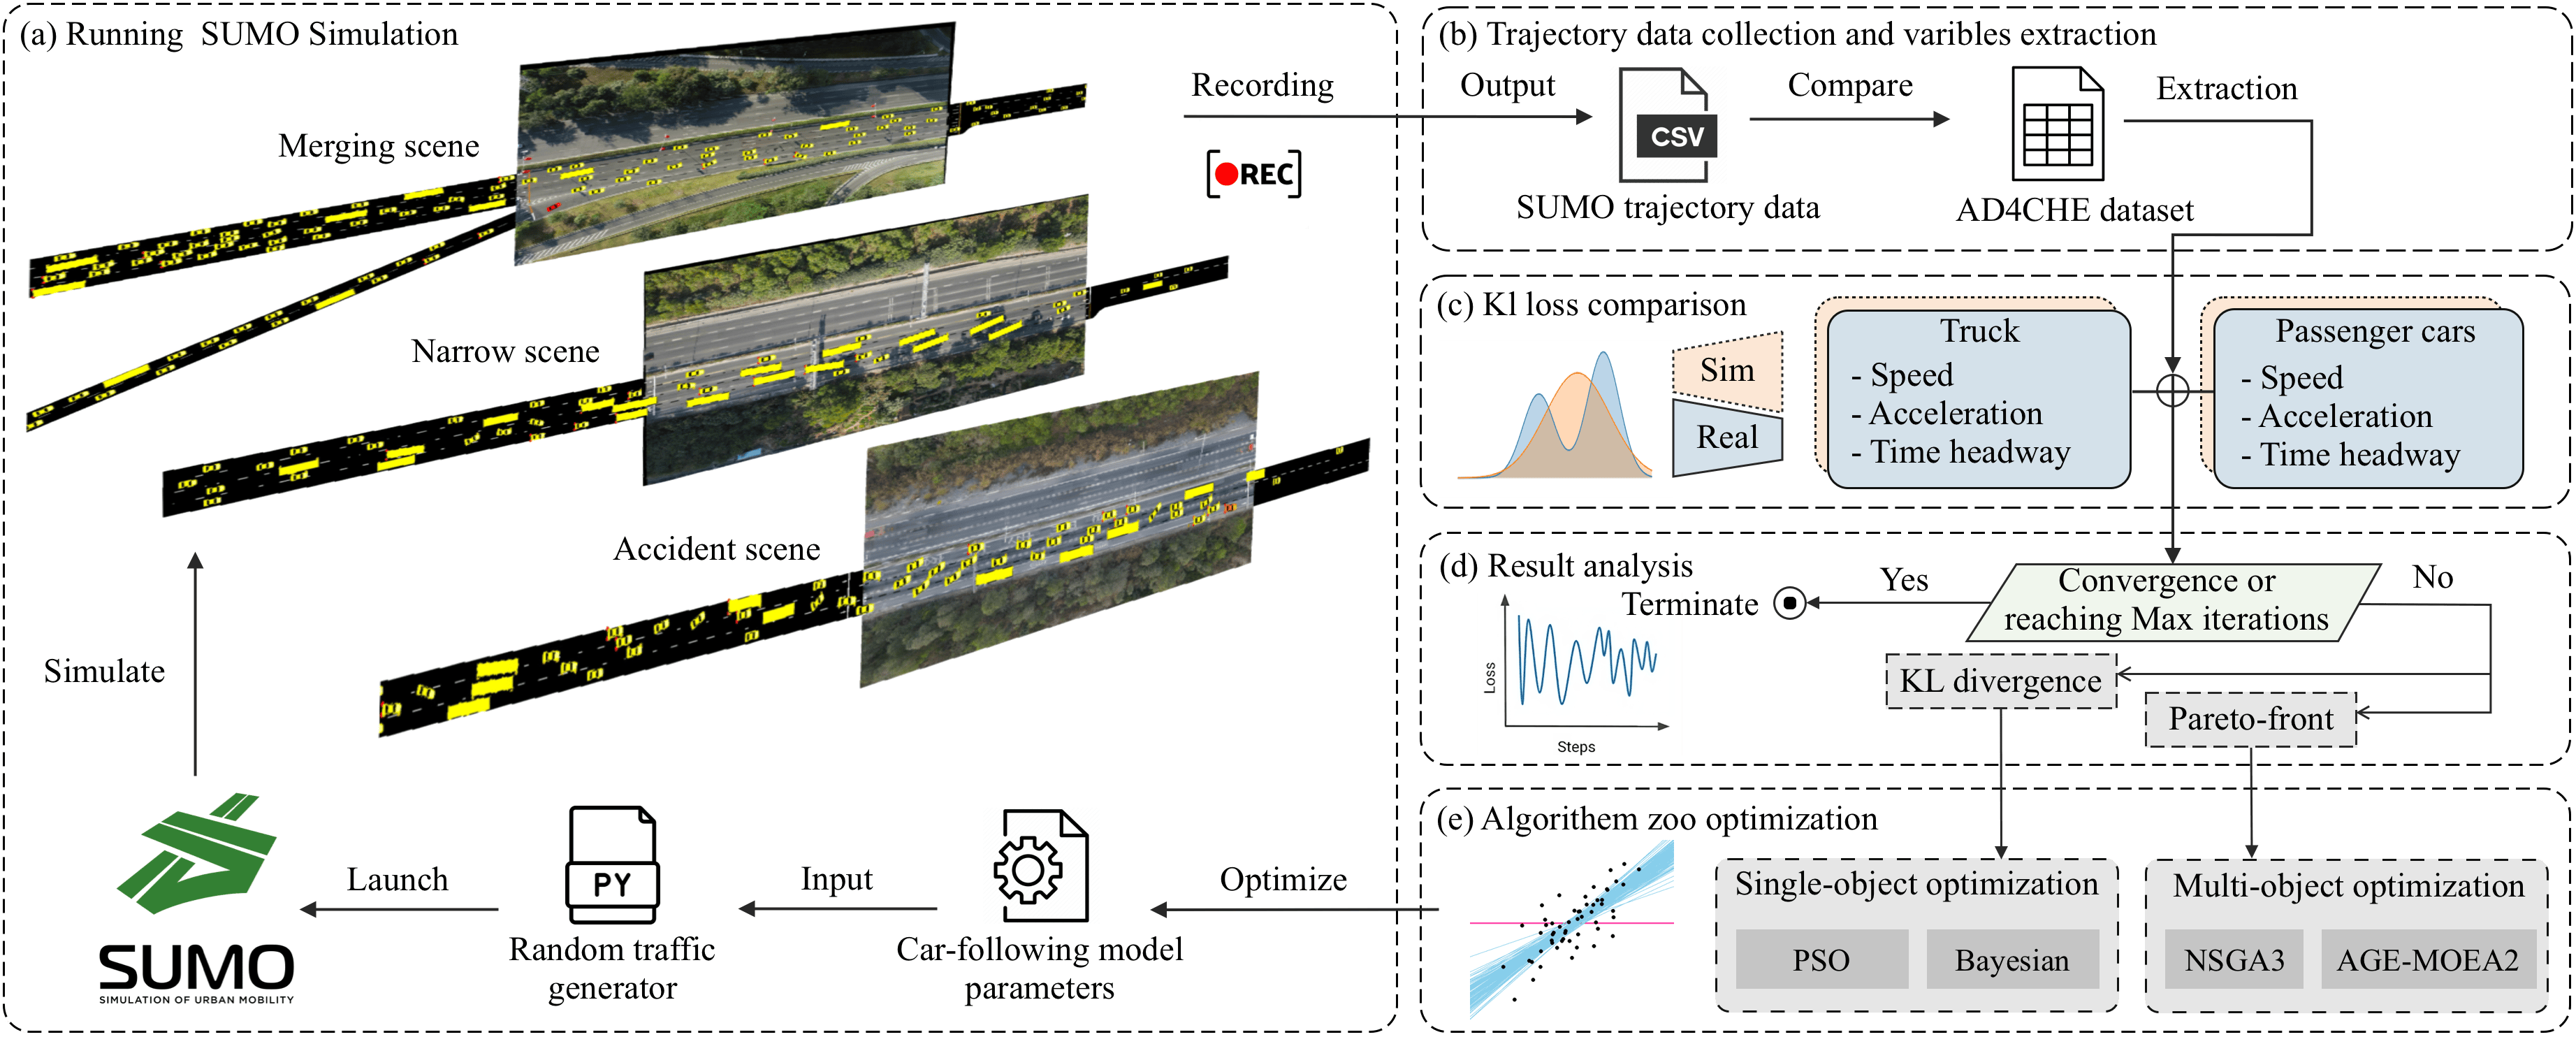
\includegraphics[width=\textwidth]{fig/calibration_framework.png}
    \caption{Calibration framework of the trustworthy traffic simulation}
    \label{fig:calibration}
\end{figure*}

\subsection{Trustworthy Traffic Scenario Generation}
To make simulation an effective tool for developing autonomous driving algorithms, the simulator needs to generate realistic traffic scenarios with precise distributions that accurately reflect the behavior of background traffic agents.

We achieve this by calibrating the parameters of EIDM \cite{EIDM} car-following models using aggregated feature distributions derived from real-world vehicle trajectory datasets as optimization targets.
Through iterative refinement of these parameter distributions, we minimize the divergence between simulated and real trajectory features, thereby generating realistic and naturally interactive driving behaviors for background traffic agents.

Fig. \ref{fig:calibration} illustrates our generation process in detail. In step (a), we run the simulator as a black-box, high-cost function in the optimization process. Specifically, the simulator can be represented as a function $f(\mathbf{x})$, where $\mathbf{x} = [x_1, x_2, \ldots, x_N]^\top$ is the vector of input parameters for the car-following model that drives the background traffic agents. These parameters are subject to the inequality constraints specified by the boundaries shown in Table \ref{tab:parameter_bounds}:


\begin{table}[ht]
\centering
\caption{Boundaries of the car-following model parameters}
\label{tab:parameter_bounds}
\begin{tabular}{p{1.2cm}p{4.5cm}p{0.9cm}p{0.9cm}}
\toprule
\multicolumn{1}{c}{\textbf{Parameters}} & \multicolumn{1}{c}{\textbf{Descriptions (Unit)}} & \multicolumn{1}{c}{\textbf{Car}} & \multicolumn{1}{c}{\textbf{Bus}} \\
\midrule                 
$\tau_{\text{mean}}$ & Average time headway (\si{\second}) & (0.5, 4) & (0.5, 4) \\
$\tau_{\text{std}}$ & Std. deviation of time headway ($-$)  & (0, 10) & (0, 10) \\
$v_{\text{mean}}$ & Average max speed (\si{\meter/\second}) & (8, 26) & (8, 26) \\
$v_{\text{std}}$ & Std. deviation of max speed ($-$) & (0, 20) & (0, 20) \\
$a$ & Max acceleration (\si{\meter/\second^{2}}) & (0.2, 4)  & (0.2, 4) \\
$d$ & Max deceleration  (\si{\meter/\second^{2}}) & (0.2, 4) & (0.2, 4) \\
$L_{\text{sublane}}$ & Eagerness to align laterally in-lane ($-$) & (0, 1) & (0, 1) \\
$L_{\text{pushy}}$ & Willingness to encroach laterally ($-$) & (0, 1) & (0, 1) \\
$L_{\text{speed\_gain}}$ & Lane-changing for speed gain ($-$) & (0, 5) & (0, 5) \\
$L_{\text{assertive}}$ & Acceptance of smaller gaps ($-$) & (1, 100) & (1, 100) \\
$L_{\text{cooperative}}$ & Cooperative lane-changing ($-$) & (0, 1) & (0, 1) \\
$L_{\text{lookahead}}$ & Adjustment for lookahead distance (\si{\meter}) & (2, 100) & (2, 100) \\
\bottomrule
\end{tabular}
\end{table}

Meanwhile, the scenario configurations, including road topology, traffic flow, and vehicle type distribution, are pre-established based on the statistical properties of the dataset.

The trajectory data generated by the simulator will undergo (b) trajectory data collection and variable extraction. This process yields aggregated distributions of variables such as speed, acceleration, and headway for different types of agents (e.g., trucks and passenger cars). Subsequently, we employ the Kullback-Leibler (KL) divergence to compare the aggregated feature distributions between the simulated and real-world data. The KL divergence for the $m$-th feature is calculated as:

\begin{equation}
D_{\mathrm{KL}}^{(m)} = \sum_{i} p_i^{(m)} \log \left( \frac{p_i^{(m)}}{q_i^{(m)}} \right),
\end{equation}

where $p_i^{(m)}$ and $q_i^{(m)}$ are the probability distributions of the $m$-th feature from the simulated data and the real data, respectively. The set of KL divergences $\{ D_{\mathrm{KL}}^{(1)}, D_{\mathrm{KL}}^{(2)}, \ldots, D_{\mathrm{KL}}^{(M)} \}$ serve as the objectives in the optimization task.

Our goal is to solve the following optimization problem:

\begin{equation}
\begin{aligned}
\min_{\mathbf{x}} \quad & \mathbf{F}(\mathbf{x}) = [D_{\mathrm{KL}}^{(1)}, D_{\mathrm{KL}}^{(2)}, \ldots, D_{\mathrm{KL}}^{(M)}], \\
\text{s.t.} \quad & x_i^{L} \leq x_i \leq x_i^{U}, \quad i = 1, \ldots, N.
\end{aligned}
\end{equation}
where $x_i^{L}$ and $x_i^{U}$ are the lower and upper bounds for the $i$-th parameter.
In step (d), result analysis, we compare the optimization outcomes with our predefined convergence criteria to determine whether to continue optimization iterations. When using multi-objective optimization, we can manually adjust the weights of each optimization objective or examine the Pareto front to understand the trade-offs between different objectives.

We utilize (e) state-of-the-art algorithms from\cite{bsy}\cite{pymoo} to optimize a new set of parameters for running the simulations.





